
% --------------------------------------------------------------- CONFIGURATIONS

\documentclass[a4paper,12pt,final,oneside]{book}

\usepackage{rapport}


% -------------------------------------------------------------- META: CONSTANTS

\newcommand{\reporttitle}{Informatique D\'ecisionnelle}
\newcommand{\enseignants}{M~\textsc{Miquel}\\A~\textsc{Tchounikine}}
\newcommand{\reportauthor}{Guillaume~\textsc{Abadie}\\Thierry~\textsc{Cantenot}\\Juliette~\textsc{Courlet}\\Rémi~\textsc{Domingues}\\Adrien~\textsc{Duffy-Coissard}\\Ahmed~\textsc{Kachkach}}
\newcommand{\reportsubject}{Livrable de projet}
\newcommand{\stagetopic}{Mortality Data Pack}
\newcommand{\dateperiod}{du 7 avril au 17 avril 2014}
\newcommand{\HRule}{\rule{\linewidth}{0.5mm}}
\setlength{\parskip}{1ex} % Espace entre les paragraphes

\hypersetup{
	pdftitle={\reporttitle},%
		pdfauthor={\reportauthor},%
		pdfsubject={\reportsubject},%
		pdfkeywords={INSA Lyon} {Mortality Data Pack} {Informatique decisionnelle}
}

\title{\reporttitle}
\author{\reportauthor}
%\setcounter{tocdepth}{4}


% ------------------------------------------------------------------------- FILE

\begin{document}


    % ------------------------------------------------------------------- HEADER

	\renewcommand{\chaptername}{} %\renewcommand{\thechapter}{}
	\renewcommand{\contentsname}{Sommaire}

	\pagestyle{empty}
	\pagenumbering{Roman}


    % ------------------------------------------------------------ HEADER: TITLE

	% Inspiré de http://en.wikibooks.org/wiki/LaTeX/Title_Creation
\begin{center}
	\begin{minipage}[t]{0.48\textwidth}
	  \begin{flushleft}
	    
\includegraphics [width=40mm]{images/logo_INSA.png} \\[0.5cm]
			INSA Lyon\\
			20, avenue Albert Einstein\\
			69621 Villeurbanne Cedex
	  \end{flushleft}
	\end{minipage}
	\begin{minipage}[t]{0.48\textwidth}
	  \begin{flushright}
	    %\includegraphics [width=60mm]{images/logo_Passau.jpg} \\[0.5cm]
	    %Universität Passau\\
		%Innstraße, 3\\
		%	D-94032 Passau
	  \end{flushright}
	\end{minipage} \\[2cm]

	\textsc{\Large \reportsubject}\\[0.3cm]
	\HRule \\[0.4cm]
	{\Huge \bfseries \reporttitle}\\[0.3cm]
	{\LARGE \bfseries «~\stagetopic~»}\\[0.3cm]
	{\Large \dateperiod}\\[0.4cm]
	\HRule \\[1cm]

	
\includegraphics [scale=0.35]{images/application-xml.png} \\[0.7cm]
	\begin{minipage}[t]{0.4\textwidth}
	  \begin{flushleft} \large
	    \emph{Hexanôme~:}\\
	    \small \reportauthor
	  \end{flushleft}
	\end{minipage}
	\begin{minipage}[t]{0.5\textwidth}
	  \begin{flushright} \large
	    \emph{Enseignants~:} \\
	    \enseignants
	  \end{flushright}
	\end{minipage}

	\vfill
	\footnotesize{Année scolaire 2013-2014}
\end{center}



    % --------------------------------------------------- HEADER: CONFIGURATIONS

	\sloppy          % Justification moins stricte : des mots ne dépasseront pas des paragraphes

    \frontmatter
		\pagestyle{empty}
		\tableofcontents
		\addtocontents{toc}{\protect\thispagestyle{empty}}

	\mainmatter
	\pagestyle{headings}

	\renewcommand{\chaptermark}[1]{\markboth{\MakeUppercase{\chaptername\ \thechapter.\ #1}}{}}
	\renewcommand{\sectionmark}[1]{\markright{\thesection{} #1}}


    % ------------------------------------------------------------------ CONTENT

    \chapter{Analyse des données}

\section{Visualisation des données}

Requête utile pour voir la répartition des causes de décés selon le sexe :

\begin{lstlisting}[frame=single, language=SQL]
SELECT sexage.SEX, causes.LABEL, COUNT(*) AS Number
FROM london INNER JOIN
        sexage ON london.SEXAGE = sexage.SEXAGE INNER JOIN
        causes on london.CAUSE = causes.CAUSE
GROUP BY sexage.sex, causes.label
\end{lstlisting}

\section{Séparation des données de sexe et d'age}

    Vu le format des données de la table SexAge, dissocier l'effet du sexe et de l'âge s'avérait hardu.

    Nous avons donc modifié la table en créant deux nouvelles colonnes: Sex, nvarchar qui contiendra le sexe (M/F), et Age,
    nvarchar qui contiendra la tranche d'âge (<1, 10-14, ...).

    Nous avons alors lancé la requête suivante afin de séparer les données de ``sexage'' sur ces deux colonnes :

    \begin{lstlisting}[frame=single, language=SQL]
UPDATE sexage
SET Sex=LEFT(label, 1), Age=RIGHT(label, LEN(label) - 1);
    \end{lstlisting}

\section{Incohérences dans les nombre de morts}

    En analysant la table des morts de chaque région, nous avons remarqué que la somme des morts par cause de niveau 2 était
    inférieure au nombre de morts par cause de niveau 1 (càd de toutes les causes de mort).

    Cette incohérence peut être montrée sur la table ``westmids'' (par exemple) avec la requête suivante :

    \begin{lstlisting}[frame=single, language=SQL]
SELECT causes.NIVEAU, SUM(westmids.DEATHS) AS TotalDeaths
FROM westmids INNER JOIN causes ON westmids;CAUSE = causes.CAUSE
GROUP BY causes.NIVEAU
HAVING (causes.NIVEAU = 1) OR (causes.NIVEAU = 2)
    \end{lstlisting}

    Ceci est probablement dû à une erreur lors du remplissage des formulaires (cause de niveau 2 non-remplie).

    La solution qu'on propose est de rajouter une nouvelle cause de mort de niveau 2 représentant une cause indéfinie, afin
    de ne pas sous-estimer le nombre de morts en ignorant ceux dont la cause de niveau 2 n'est pas renseignée.

    \begin{lstlisting}[frame=single, language=SQL]
METTRE LES REQUETES QUI VONT BIEN ICI
    \end{lstlisting}

\section{Union des données dans une nouvelle table}

    TODO : Mettre du blabla aussi.

    \begin{lstlisting}[frame=single, language=SQL]
INSERT INTO deaths
SELECT *
FROM
(
    SELECT * FROM london UNION
    SELECT * FROM mersey UNION
    SELECT * FROM yorkhumb UNION
    SELECT * FROM ntheast UNION
    SELECT * FROM nthwest UNION
    SELECT * FROM stheast UNION
    SELECT * FROM sthwest UNION
    SELECT * FROM eastern UNION
    SELECT * FROM eastminds UNION
    SELECT * FROM wales UNION
    SELECT * FROM westmids UNION
)
    \end{lstlisting}


\section{Visualisation des données}

    Nous avons exploré les données mises à notre disposition, en essayant de trouver des motifs, incohérences et autres motifs particuliers
    dans ces dernières.

    Pour cela, nous avons effectué plusieurs requêtes SQL, comme cette requête qui donne la répartition des décès par sexe pour chaque
    cause.

    \begin{lstlisting}[frame=single, language=SQL]
SELECT sexage.SEX, causes.LABEL, COUNT(*) AS Number
FROM london INNER JOIN
        sexage ON london.SEXAGE = sexage.SEXAGE INNER JOIN
        causes on london.CAUSE = causes.CAUSE
GROUP BY sexage.sex, causes.label
    \end{lstlisting}

    On a donc découvert que, surprise !, il n'y a pas de décès ayant pour cause un avortement chez le sexe masculin.
    \chapter{\textit{Reporting}}


====> Lien intéressant pour tous (office national de statistiques pour les UK, avec un tas de diagrammes complets et intéressants) : http://www.ons.gov.uk

\section{Cube patate}


Le lien ci-dessous peut être utile : graphique d'évolution des conditions sanitaires (health) pour les différentes classes de population par famille de cluster

\begin{verbatim}
http://www.google.fr/url?sa=t&rct=j&q=&esrc=s&source=web&cd=4&ved=0CEoQFjAD&url=http%3A%2F%2Fwww.ons.gov.uk%2Fons%2Fguide-method%2Fgeography%2Fproducts%2Farea-classifications%2Fns-area-classifications%2Findex%2Fcluster-summaries%2Fhealth-areas%2Fprospering-uk.pdf&ei=LodSU-raKqiZ0QXjr4CwDw&usg=AFQjCNESWJHRf0se4ScTkOhLLWBMoYvW3g&sig2=PxLbntsqK0DGj7pG3Us-Kw&bvm=bv.65058239,d.d2k
\end{verbatim}

\subsection{Troubles mentaux, et évolution de leur prise en charge}

    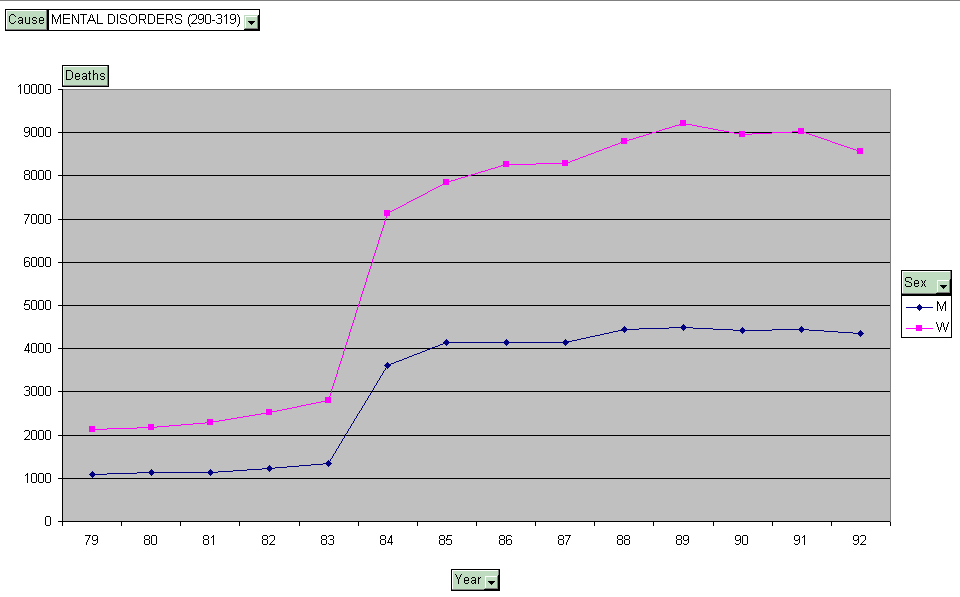
\includegraphics[scale=0.5]{images/mental_disorder.png}

    Une cause de mort a attiré notre attention plus que les autres~: les ``mental disorder''. En plus de présenter une grande disparité
    entre morts chez les hommes et les femmes, le nombre morts causées par ces troubles a drastiquement augmenté en 1983.

    Nous avons essayé de chercher des signes d'une augmentation aussi drastique des morts chez les autres causes, en vain. Il était donc
    clair que cette augmentation était bien spécifique aux \textit{troubles mentaux}.

    Nous sommes donc allés chercher les événements marquants s'étant produits en Grande-Bretagne autour de 1983, et quelques recherches
    et articles plus tard, nous avons isolé la cause à l'origine de cette hausse : le \href{en.wikipedia.org/wiki/Mental_Health_Act_1983‎}{Mental Health Act of 1983}.

    Cet acte parlementaire a introduit une nouvelle classification des \textit{troubles mentaux} et un traitement

\subsection{Morts néonatales et nouveaux certificats de décès}

    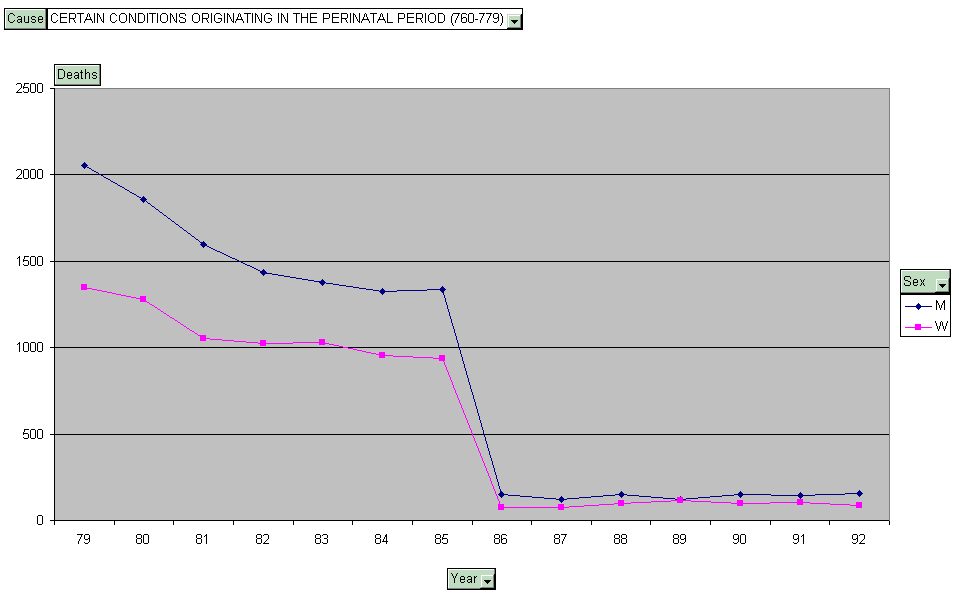
\includegraphics[scale=0.5]{images/perinatal.png}

    Blah blah.

\subsection{Maladies musculo-squelettique}

    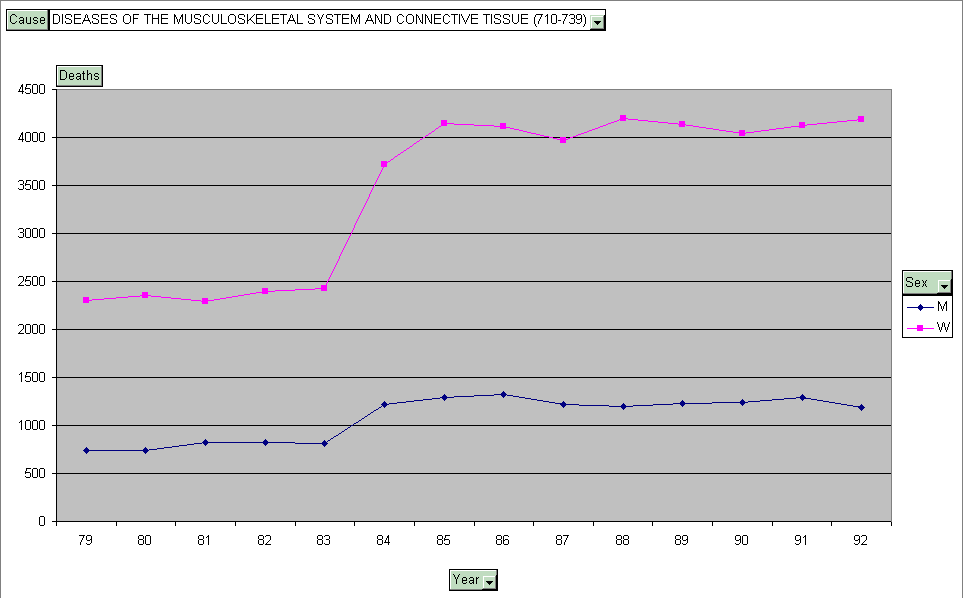
\includegraphics[scale=0.5]{images/muscoskeletal.png}

    Blah blah.

\pagebreak


\section{Cube Population}
\subsection{Évolution de la population au cours du temps}
\begin{figure}[h!]
    \centering
    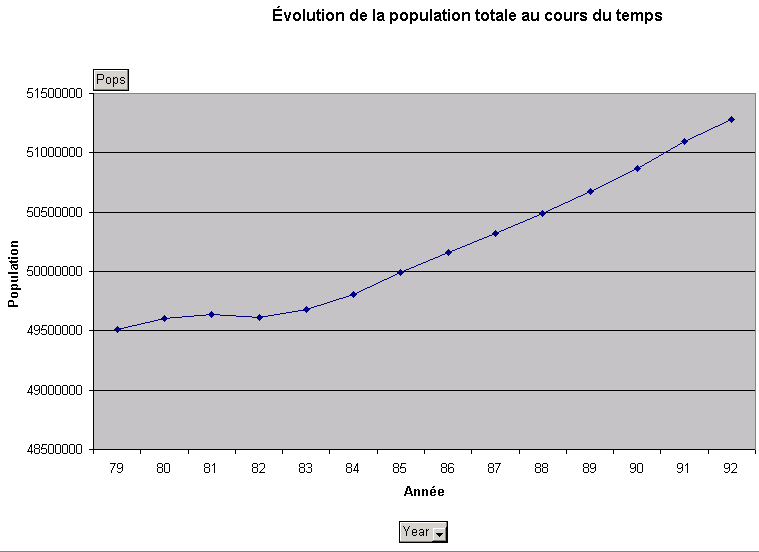
\includegraphics[width=\linewidth]{images/pop/evolutionPopulation.png}
\end{figure}

Le graphique précédent illustre la croissange démographique générale des Royaumes Unis entre 1972 et 1992. Cette courbe est en accord avec celles d'autres pays occidentaux à la même époque, la croissance démographique étant ici linéaire et en faible progression.

On notera que les relevés de population précédant l'année 1981 diffèrent de par la technique de comptage effectué. Avant cette date, les touristes présents aux Royaumes Unis étaient comptabilisés dans les données de population, alors que les résidents qui étaient hors du territoire à la date de rencencement ne l'étaient pas. À compter de 1981, les touristes n'étant plus comptés, et les résidents l'étant, ceci explique l'allure légèrement décroissante de la courbe entre 1981 et 1982.

On observe alors une population résidente d'environ 49 650 000 personnes en 1982, ce chiffre culminant à 51 300 000 personnes en 1992, soit une croissance d'environ 3.32\% (+1 650 000 résidents) en 10 ans.
\pagebreak


\subsection{Évolution de la répartition hommes / femmes au cours du temps}
\begin{figure}[h!]
    \centering
    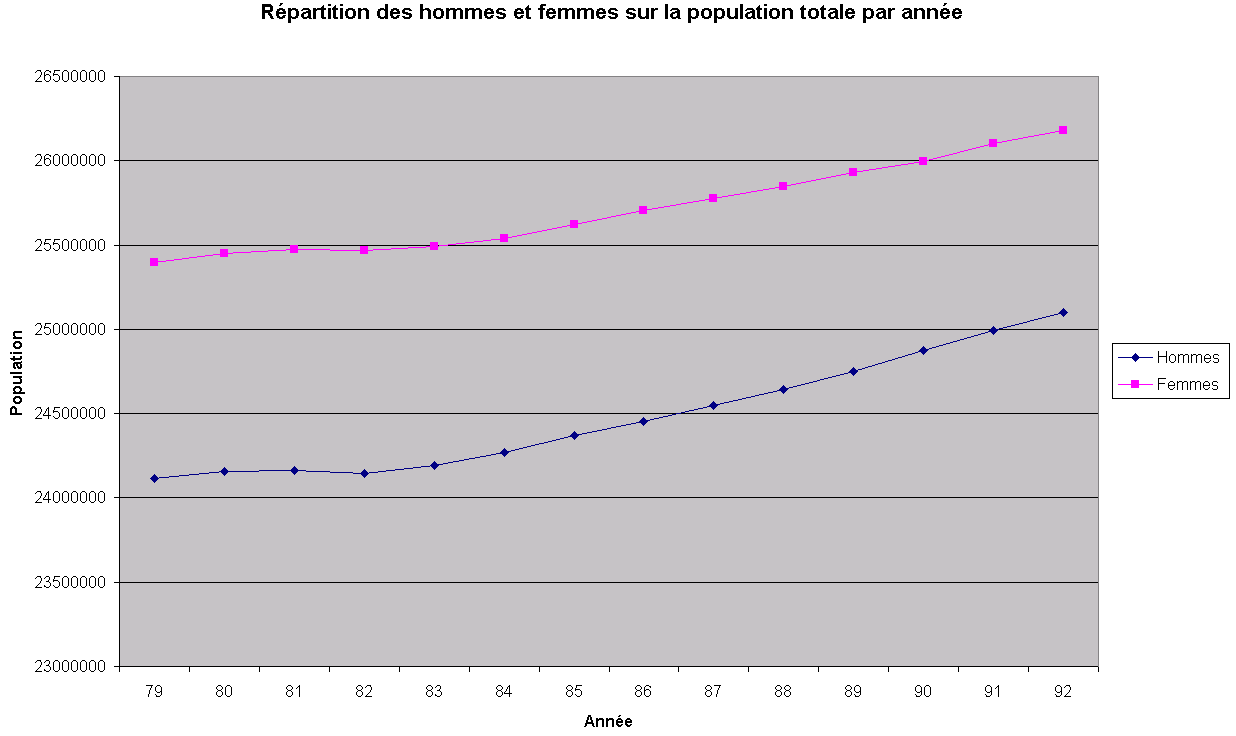
\includegraphics[width=\linewidth]{images/pop/repartitionHF.png}
\end{figure}

On peut ici observer que la répartition hommes / femmes est restée constante au cours du temps, l'allure d'une courbe épousant aisément celle de l'autre.

On dénote près de 24.2 millions d'hommes et 25.5 millions de femmes aux Royaumes Unis en 1982 contre respectivement 25.1 et 26.2 millions en 1991.

Ceci représente une croissance de 3.72\% (+0.9 millions) chez les hommes et 2.75\% (+0.7 millions) chez les femmes.

La croissance démographique est donc plus grande chez les hommes que chez les femmes.
\pagebreak


\subsection{Répartition de la population par classes d'âge en 1992}
\begin{figure}[h!]
    \centering
    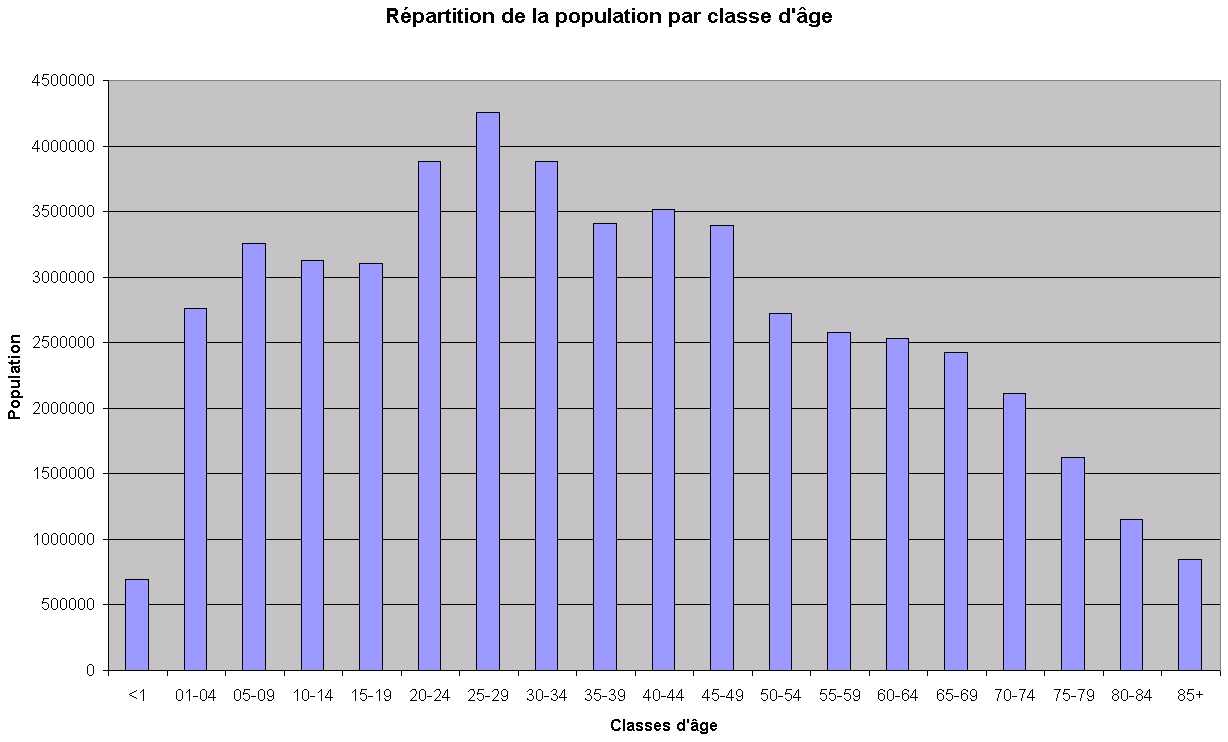
\includegraphics[width=\linewidth]{images/pop/pyramideAges.png}
\end{figure}

En accord avec les répartitions par classes d'âges des pays européens à cette époque, le graphique ci-dessus illustre une pyramide des âges tout à fait standard pour un pays développé.
\pagebreak


\subsection{TODO}
=> => => Répartition de la population par région / cluster manquante !!!!!
\pagebreak


\subsection{Déplacements de population par région}
\begin{figure}[h!]
    \centering
    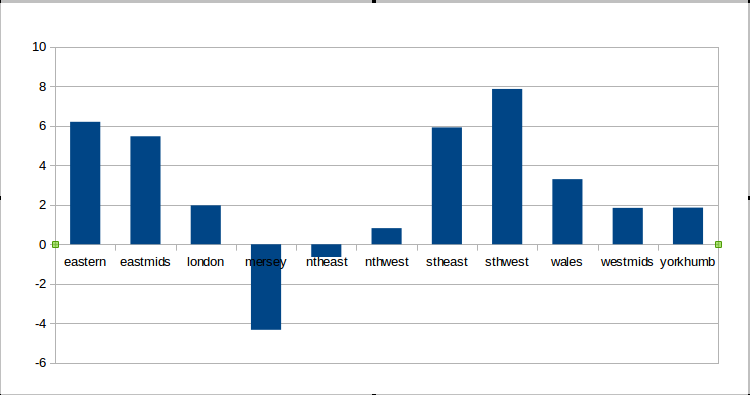
\includegraphics[width=\linewidth]{images/pop/deltaPopRegions.png}
\end{figure}
TODO : Adrien
=> => => WARNING : On est parti de 1981 pour les données, alors que 1981 est encore erronée ! Il aurait fallu partir de 1982
\pagebreak


\subsection{Déplacements de population par famille de clusters}
=> => => WARNING : On est parti de 1981 pour les données, alors que 1981 est encore erronée ! Il aurait fallu partir de 1982

\begin{figure}[h!]
    \centering
    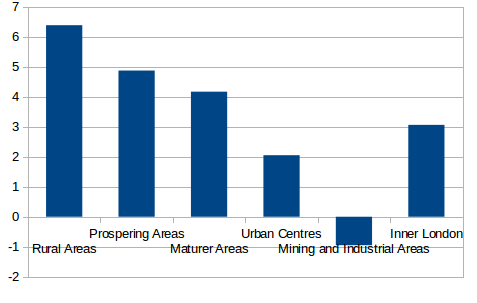
\includegraphics[width=\linewidth]{images/pop/deltaPopFamilleCluster.png}
\end{figure}

On observe ici les effets d'une exode rurale toujours présente au cours des dernières années, la population urbaine tendant à retourner au sein du milieu rural. En effet, si la population tend à croître dans les milieux urbains (+220 000 personnes pour les centres urbains, et +90 000 pour le centre londonien) et ruraux (+600 000 personnes), sa croissance est bien plus forte pour les zones rurales, dénotant un déplacement de population certain au cours des 10 années d'étude.

Ce déplacement est d'autant plus visible au sein des milieux miniers et industriels, les zones rattachées au secteur secondaire observant une diminution de près de 130 000 personnes.
\pagebreak


\subsection{}
\begin{figure}[h!]
    \centering
    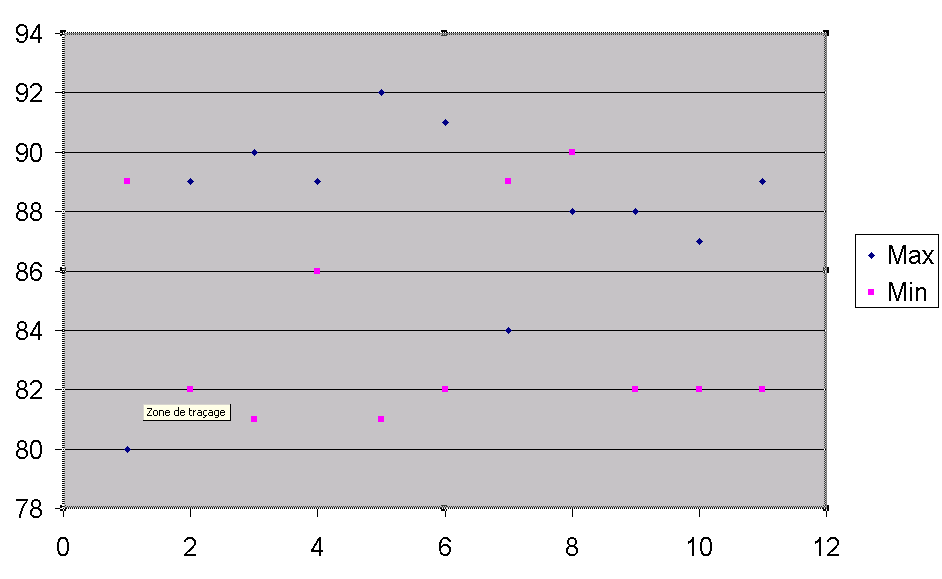
\includegraphics[width=\linewidth]{images/pop/anneeMinMax(TODO).png}
\end{figure}
=> => => Schéma non exploitable pour l'instant
TODO : Adrien
=> => => WARNING : Débuter l'étude à partir de 1982, et non 1978


	%\renewcommand{\chaptermark}[1]{\markboth{\MakeUppercase{#1}}{}}
	%\renewcommand{\sectionmark}[1]{\markright{#1}}

	%\addcontentsline{toc}{part}{Annexes}
	%\part*{Annexes}
	%\appendix
	%\include{implementationExercices}


    % ------------------------------------------------------------------- FOOTER
\end{document}
